\section{Các phương pháp cải tiến}
\subsection{Cửa sổ trượt (Sliding Window)}

Cửa sổ trượt là một kỹ thuật quan trọng trong việc xử lý dữ liệu chuỗi thời gian, đặc biệt khi làm việc với các mô hình học máy yêu cầu dữ liệu có cấu trúc dạng chuỗi (sequence). Kỹ thuật này giúp chia nhỏ dữ liệu lớn thành các chuỗi con với chiều dài cố định, giúp mô hình dễ dàng học được các đặc trưng từ các chuỗi dữ liệu liên tục.

\begin{figure}[H]
    \centering
    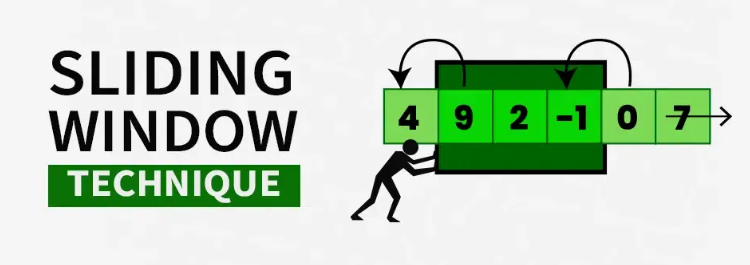
\includegraphics[width=\textwidth,height=\textheight,keepaspectratio]{Images/Improved methods/SlidingWindowTechnique.png}
    \caption{Kỹ thuật Sliding Window}
    \label{fig:enter-label}
\end{figure}

\subsubsection{Khái niệm về cửa sổ trượt}

Cửa sổ trượt sử dụng một cửa sổ cố định để trượt qua dữ liệu chuỗi thời gian, tạo ra các phân đoạn nhỏ (windows) để mô hình học máy có thể xử lý. Mỗi cửa sổ trượt chứa một số mẫu nhất định, được gọi là \textit{sequence length}. Khi cửa sổ trượt di chuyển qua dữ liệu, các mẫu trong mỗi cửa sổ được sử dụng để huấn luyện mô hình.

\begin{itemize}
    \item \textbf{Sequence length:} Số lượng mẫu trong mỗi cửa sổ.
    \item \textbf{Step size:} Số mẫu mà cửa sổ trượt di chuyển qua mỗi lần.
\end{itemize}

\subsubsection{Cách thức hoạt động của cửa sổ trượt}

Cửa sổ trượt hoạt động theo cách chia dữ liệu thành các cửa sổ nhỏ, mỗi cửa sổ chứa một chuỗi thời gian dài một số bước thời gian xác định. Sau đó, cửa sổ này di chuyển qua các bước tiếp theo để tạo ra các mẫu huấn luyện liên tiếp.

\begin{itemize}
    \item Dữ liệu gốc có dạng chuỗi thời gian dài $(T)$.
    \item Cửa sổ trượt có kích thước cố định (ví dụ: 240 bước thời gian).
    \item Mỗi lần trượt, cửa sổ di chuyển qua một bước xác định (step size, ví dụ: 40 mẫu).
\end{itemize}

\begin{figure}[H]
    \centering
    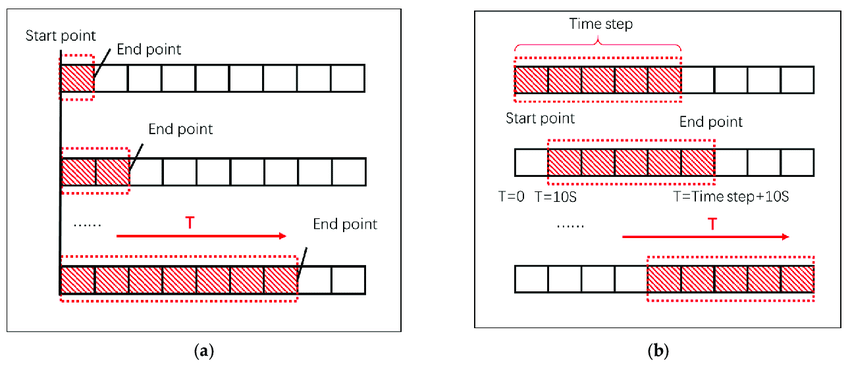
\includegraphics[width=\textwidth,height=\textheight,keepaspectratio]{Images/Improved methods/sliding-window-method.png}
    \caption{Cách thức hoạt động của Sliding Window}
    \label{fig:enter-label}
\end{figure}

\textbf{Ví dụ:}  
Giả sử chúng ta có dữ liệu chuỗi thời gian dài 1000 mẫu và cửa sổ trượt có kích thước 240 mẫu. Cửa sổ trượt sẽ tạo ra các mẫu huấn luyện sau:
\begin{itemize}
    \item Cửa sổ đầu tiên chứa mẫu 1 đến mẫu 240.
    \item Cửa sổ thứ hai chứa mẫu 41 đến mẫu 280 (di chuyển 40 mẫu).
    \item Cửa sổ thứ ba chứa mẫu 81 đến mẫu 320, và cứ thế tiếp tục.
\end{itemize}

\subsubsection{Ứng dụng cửa sổ trượt trong dự đoán}

Khi mô hình được huấn luyện xong, cửa sổ trượt sẽ được sử dụng để xử lý các dữ liệu đầu vào mới trong quá trình dự đoán, giúp mô hình nhận diện và dự đoán các cử chỉ ngôn ngữ ký hiệu một cách chính xác.

\begin{itemize}
    \item Dữ liệu đầu vào cho dự đoán sẽ được chia thành các cửa sổ thời gian với kích thước cố định, giống như trong quá trình huấn luyện.
    \item Mỗi cửa sổ sẽ chứa một chuỗi dữ liệu mới từ các cảm biến, với chiều dài cửa sổ cố định (ví dụ: 240 bước thời gian).
    \item Cửa sổ trượt di chuyển qua dữ liệu mới để tạo ra các mẫu cho mô hình dự đoán.
\end{itemize}

\textbf{Ví dụ:} Giả sử mô hình đã được huấn luyện và bây giờ cần dự đoán cho dữ liệu mới. Nếu cửa sổ trượt có kích thước 240 và bước trượt là 40 mẫu:
\begin{itemize}
    \item Cửa sổ đầu tiên chứa các mẫu từ 1 đến 240.
    \item Cửa sổ thứ hai chứa mẫu từ 41 đến 280, và cứ thế tiếp tục.
    \item Mỗi cửa sổ được đưa vào mô hình để dự đoán giá trị, sau đó mô hình sẽ trả về kết quả cho mỗi cửa sổ.
\end{itemize}

Dữ liệu được xử lý qua các cửa sổ trượt sẽ giúp mô hình dự đoán các cử chỉ theo từng chuỗi thời gian liên tiếp, từ đó tạo ra kết quả chính xác hơn và liên tục, đặc biệt khi dữ liệu mới được thu thập từ các cảm biến.

\subsubsection{Lợi ích của cửa sổ trượt trong dự đoán}

\begin{itemize}
    \item \textbf{Dự đoán liên tục:} Cửa sổ trượt giúp mô hình duy trì khả năng dự đoán liên tục cho dữ liệu chuỗi thời gian mới, không bị gián đoạn.
    \item \textbf{Giữ lại thông tin trong các chuỗi thời gian dài:} Mỗi cửa sổ giúp mô hình nắm bắt thông tin từ các bước thời gian liên tiếp, từ đó cải thiện độ chính xác của dự đoán.
    \item \textbf{Xử lý dữ liệu theo thời gian thực:} Cửa sổ trượt cho phép mô hình xử lý dữ liệu theo dạng chuỗi thời gian liên tục, giúp mô hình thích ứng với các thay đổi trong dữ liệu theo thời gian.
\end{itemize}

\subsection{Khôi phục dữ liệu bị mất}

Trong quá trình truyền dữ liệu qua Bluetooth, đặc biệt với các tín hiệu liên tục như từ cảm biến, có thể xảy ra hiện tượng mất gói dữ liệu. Điều này ảnh hưởng đến chất lượng và tính liên tục của thông tin đầu vào cho mô hình học máy. Dưới đây là các phương pháp xử lý và khôi phục dữ liệu bị mất trong quá trình truyền.

\begin{figure}[H]
    \centering
    
\includegraphics[width=0.5\textwidth,height=\textheight,keepaspectratio]{Images/Improved methods/bluetooth.png}
    \caption{Truyền dữ liệu bằng bluetooth}
    \label{fig:enter-label}
\end{figure}

\subsubsection{Nguyên nhân gây mất dữ liệu}
\begin{itemize}
    \item \textbf{Giới hạn băng thông của Bluetooth:} Khi tốc độ truyền vượt quá khả năng xử lý của kênh truyền, một số gói dữ liệu có thể bị bỏ qua.
    \item \textbf{Nhiễu tín hiệu:} Các tín hiệu không mong muốn trong môi trường có thể gây lỗi truyền dữ liệu.
    \item \textbf{Khoảng cách truyền:} Khoảng cách giữa thiết bị gửi và nhận quá xa dẫn đến tín hiệu yếu, gây mất dữ liệu.
    \item \textbf{Quá tải bộ đệm:} Dữ liệu được gửi quá nhanh khiến bộ đệm của thiết bị nhận không xử lý kịp thời.
\end{itemize}

\subsubsection{Phương pháp phát hiện dữ liệu bị mất}
\begin{itemize}
    \item \textbf{Kiểm tra tính liên tục của chuỗi dữ liệu:}  
    Mỗi gói dữ liệu được đánh số tuần tự (\textit{sequence number}). Khi phát hiện số thứ tự không liên tiếp, xác định đã có dữ liệu bị mất.
    
    \item \textbf{Kiểm tra tính đầy đủ của gói dữ liệu:}  
    Dựa vào định dạng dữ liệu cố định, nếu số lượng giá trị trong gói không khớp với định dạng chuẩn (ví dụ: thiếu 7 giá trị từ cảm biến), xác định gói bị lỗi.
\end{itemize}

\subsubsection{Phương pháp khôi phục dữ liệu bị mất}
\begin{enumerate}
    \item \textbf{Nội suy tuyến tính (Linear Interpolation):}
    \begin{itemize}
        \item Áp dụng khi mất một số ít gói dữ liệu liên tiếp.
        \item Dựa vào giá trị của các gói trước và sau gói bị mất để tính toán giá trị trung bình hoặc ước lượng dữ liệu:
        \[
        x_{\text{khôi phục}} = x_{\text{trước}} + \frac{x_{\text{sau}} - x_{\text{trước}}}{\Delta t}
        \]
        \item Phương pháp này đảm bảo tín hiệu khôi phục mượt mà và duy trì tính liên tục.
    \end{itemize}
    
    \item \textbf{Sao chép giá trị gần nhất (Forward/Backward Filling):}
    \begin{itemize}
        \item Áp dụng cho các trường hợp mất dữ liệu ngắn.
        \item Giá trị bị mất được thay thế bằng giá trị gần nhất (trước hoặc sau gói bị mất).
        \item Phương pháp này đơn giản và hiệu quả khi dữ liệu thay đổi ít theo thời gian.
    \end{itemize}
    
    \item \textbf{Bổ sung giá trị mặc định:}
    \begin{itemize}
        \item Áp dụng khi không thể nội suy do mất nhiều gói liên tiếp hoặc không có dữ liệu tham chiếu.
        \item Giá trị bị mất được thay bằng giá trị mặc định (ví dụ: 0 hoặc giá trị trung bình của chuỗi).
    \end{itemize}
    
    \item \textbf{Yêu cầu gửi lại dữ liệu:}
    \begin{itemize}
        \item Trong trường hợp quan trọng, thiết bị nhận có thể gửi tín hiệu yêu cầu thiết bị gửi phát lại gói bị mất.
        \item Phương pháp này hiệu quả nhưng tăng độ trễ trong hệ thống.
    \end{itemize}
\end{enumerate}

\subsubsection{Tối ưu hóa giảm thiểu mất dữ liệu}
\begin{itemize}
    \item \textbf{Điều chỉnh tốc độ truyền:} Giảm tốc độ truyền để phù hợp với khả năng xử lý của thiết bị nhận.
    \item \textbf{Sử dụng nén dữ liệu:} Nén tín hiệu để giảm kích thước gói, tăng tốc độ truyền.
    \item \textbf{Giảm nhiễu tín hiệu:} Sử dụng các kênh tần số khác hoặc cải thiện điều kiện môi trường truyền dữ liệu.
    \item \textbf{Tăng độ nhạy Bluetooth:} Đảm bảo khoảng cách giữa thiết bị gửi và nhận nằm trong giới hạn hỗ trợ của Bluetooth.
\end{itemize}





\subsection{Cải thiện chất lượng mô hình}
\subsubsection{Mô hình với Deep Convolution và Self-Attention}

Trong đề tài trước, mô hình học máy được sử dụng khá thô sơ và đơn giản, bao gồm các thành phần chính: một lớp \textit{LSTM}, một lớp \textit{Dropout}, một lớp \textit{Flatten}, và hai lớp \textit{Dense}. 

\begin{figure}[H]
    \centering
    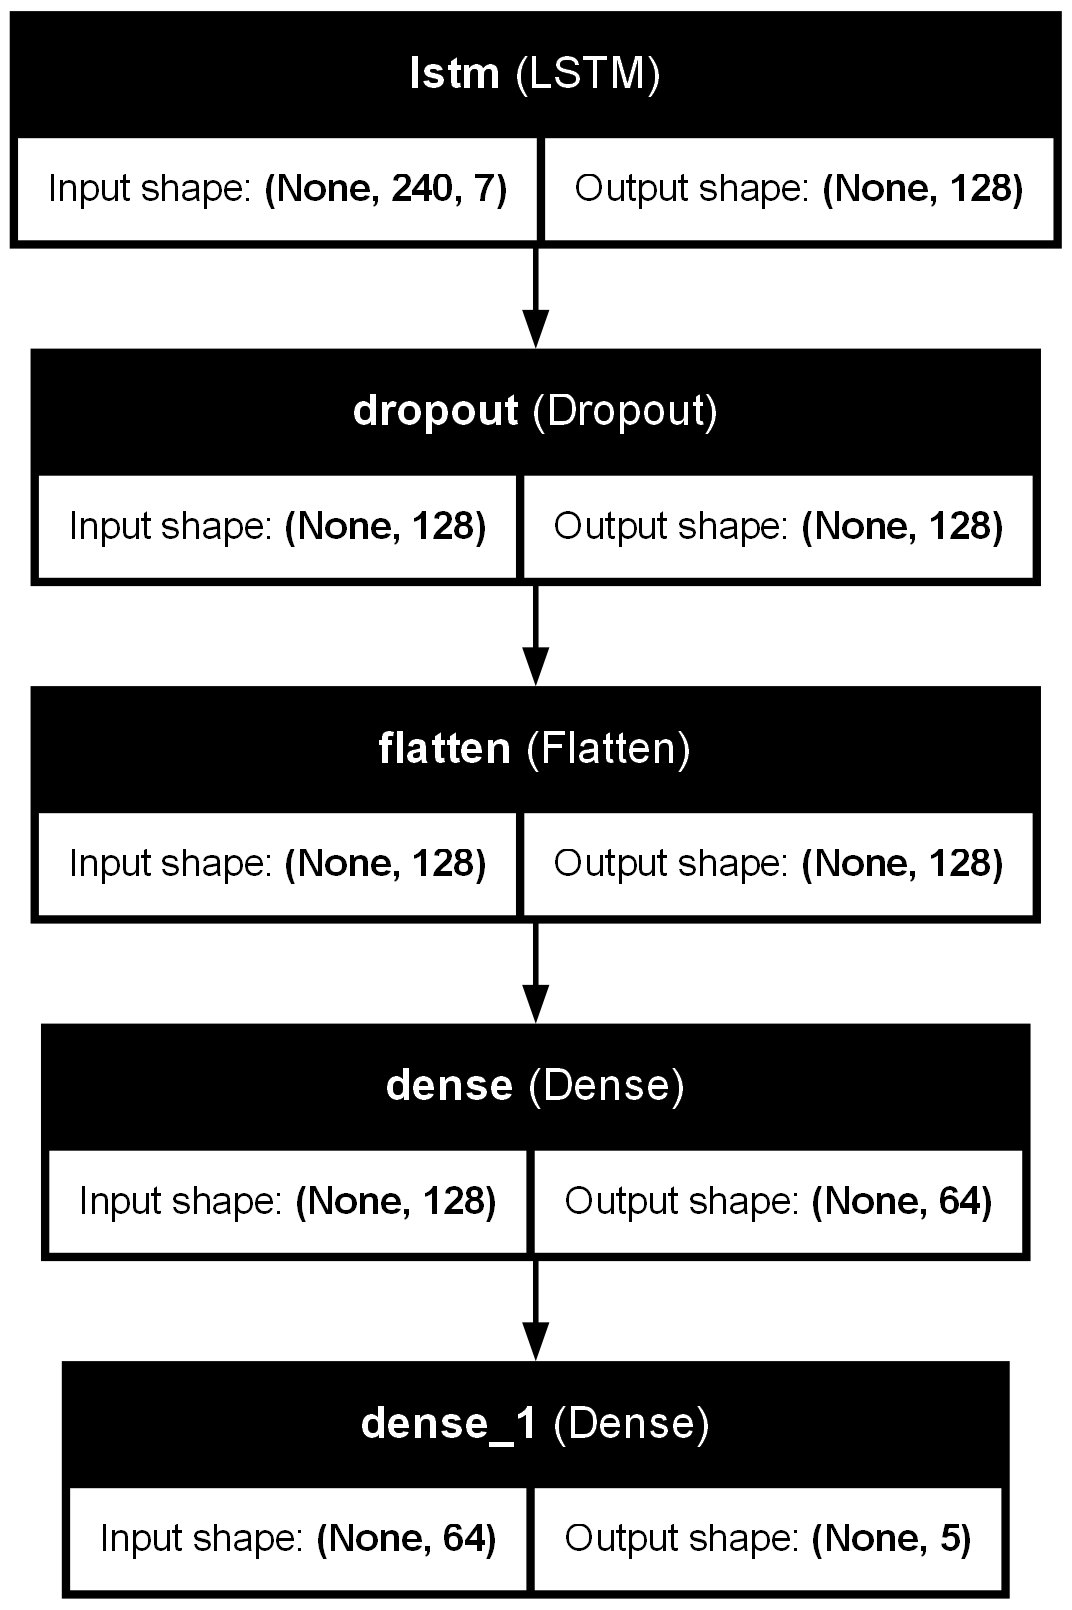
\includegraphics[width=0.5\linewidth]{Images/Improved methods/old_model_plot.png}
    \caption{Cấu trúc mô hình cũ}
    \label{fig:old-model}
\end{figure}

Kết quả đạt được từ mô hình này vẫn chưa thực sự khả quan. Để cải thiện chất lượng đầu ra, cần thực hiện hai bước quan trọng:
\begin{itemize}
    \item \textbf{Gia tăng kích thước tập dữ liệu}: Mở rộng và đa dạng hóa dữ liệu đầu vào.
    \item \textbf{Nâng cấp mô hình}: Sử dụng kiến trúc học máy hiệu quả hơn để khai thác triệt để thông tin từ dữ liệu.
\end{itemize}

Trong đề tài này, nhóm đề xuất một mô hình cải tiến, dựa trên kiến trúc được giới thiệu trong bài báo \textit{"Self-Attention-Based Deep Convolution LSTM Framework for Sensor-Based Badminton Activity Recognition"} (\href{https://doi.org/10.3390/s23208373}{DOI: 10.3390/s23208373}). Mô hình này kết hợp:
\begin{enumerate}
    \item \textbf{Mạng nơ-ron tích chập (CNN)}: Chiết xuất các đặc trưng cục bộ từ dữ liệu đầu vào.
    \item \textbf{Mạng nơ-ron hồi quy (LSTM)}: Nắm bắt các phụ thuộc dài hạn trong dữ liệu.
    \item \textbf{Cơ chế Self-Attention}: Tập trung vào các phần quan trọng nhất của dữ liệu.
\end{enumerate}

Mô hình đề xuất bao gồm các thành phần chính sau:
\begin{itemize}
    \item \textbf{Lớp CNN}: Chiết xuất các đặc trưng cục bộ từ dữ liệu đầu vào.
    \item \textbf{Lớp LSTM}: Nắm bắt và lưu giữ các thông tin phụ thuộc dài hạn trong chuỗi thời gian.
    \item \textbf{Cơ chế Self-Attention}: Xác định và tập trung vào các đặc trưng quan trọng nhất trong dữ liệu, cải thiện hiệu quả học hỏi của mô hình.
\end{itemize}

\begin{figure}[H]
    \centering
    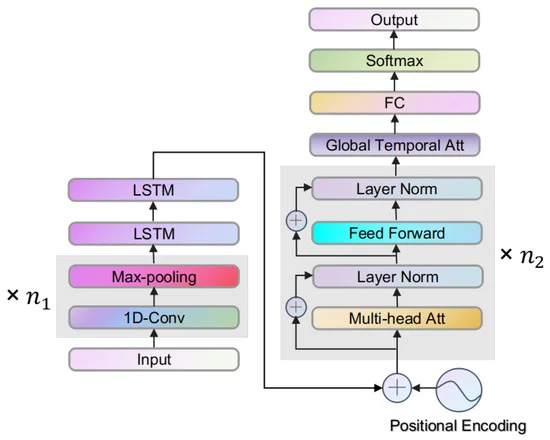
\includegraphics[width=0.8\linewidth]{Images/Architecture/SADeepConv.png}
    \caption{Mô hình mới}
    \label{fig:new-model}
\end{figure}


\noindent
Cơ chế \textit{Self-Attention} đóng vai trò then chốt trong việc nâng cao hiệu suất của mô hình. Nó cho phép mô hình tự động:
\begin{itemize}
    \item Phân tích toàn bộ dữ liệu đầu vào.
    \item Tập trung vào những đặc trưng mang tính quyết định.
\end{itemize}

Nhờ vậy, mô hình có thể đạt được độ chính xác cao hơn trong việc dự đoán các hành động theo chuỗi thời gian.

\subsection{Làm giàu dữ liệu}
\subsubsection{Data Augmentation}

Trong học máy, \textit{Data Augmentation} là một kỹ thuật quan trọng giúp mở rộng tập dữ liệu hiện có bằng cách tạo ra các biến thể mới của dữ liệu. Điều này không chỉ cải thiện tính đa dạng của dữ liệu mà còn giúp mô hình giảm thiểu hiện tượng quá khớp (\textit{overfitting}) và học được nhiều đặc trưng tổng quát hơn. Dưới đây là một số kỹ thuật được áp dụng:

\begin{enumerate}

\item \textbf{Jittering}: 
\begin{itemize}
\item \textbf{Mô tả}: Thêm nhiễu ngẫu nhiên vào dữ liệu. Jittering có thể được thực hiện bằng cách thêm một lượng nhỏ nhiễu Gaussian vào mỗi điểm dữ liệu. Điều này giúp mô hình ít bị ảnh hưởng bởi nhiễu trong dữ liệu thực tế và tăng khả năng kháng nhiễu của mô hình.
\item \textbf{Lợi ích}: 
\begin{itemize}
\item Giúp mô hình trở nên mạnh mẽ hơn trước các biến động nhỏ trong dữ liệu thực tế.
\item Tăng khả năng tổng quát hóa bằng cách làm cho dữ liệu đầu vào đa dạng hơn.
\end{itemize}
\end{itemize}

\item \textbf{Scale}: 
\begin{itemize}
\item \textbf{Mô tả}: Thay đổi tỷ lệ của dữ liệu. Scale được thực hiện bằng cách nhân mỗi điểm dữ liệu với một hệ số tỷ lệ ngẫu nhiên.
 \item \textbf{Lợi ích}:
\begin{itemize}
\item Giúp mô hình học được các đặc trưng ở các mức độ hoặc tỉ lệ khác nhau.
 \item Phù hợp với các bài toán mà dữ liệu có sự biến thiên về kích thước, chẳng hạn như tín hiệu sinh lý.
\end{itemize}
 \end{itemize}

\item \textbf{Magnitude Warp}: 
\begin{itemize}
\item \textbf{Mô tả}: Biến dạng biên độ của dữ liệu theo một hàm phi tuyến. Magnitude Warp có thể được thực hiện bằng cách áp dụng một hàm phi tuyến, chẳng hạn như hàm sin hoặc hàm mũ, cho biên độ của dữ liệu.
\item \textbf{Lợi ích}:
\begin{itemize}
\item Tạo ra các biến thể tín hiệu thực tế hơn, đặc biệt phù hợp với các bài toán liên quan đến chuỗi thời gian.
\item Làm phong phú tập dữ liệu và giúp mô hình ít phụ thuộc vào các dạng tín hiệu cụ thể.
 \end{itemize}
\end{itemize}

\item \textbf{Shift}: 
 \begin{itemize}
 \item \textbf{Mô tả}: Dịch chuyển dữ liệu theo thời gian. Shift được thực hiện bằng cách dịch chuyển toàn bộ chuỗi thời gian sang trái hoặc phải một khoảng thời gian ngẫu nhiên.
 \item \textbf{Lợi ích}:
\begin{itemize}
\item Tăng khả năng chống lại sự thay đổi vị trí trong dữ liệu, chẳng hạn như các tín hiệu không đồng bộ.
\item Giúp mô hình học được các đặc trưng không bị phụ thuộc vào vị trí cụ thể.
\end{itemize}
\end{itemize}

\end{enumerate}

Để tăng cường dữ liệu huấn luyện, nhóm đã xây dựng một script Python để áp dụng các kỹ thuật Data Augmentation đã đề cập ở trên. Script này nhận dữ liệu gốc làm đầu vào và tạo ra các phiên bản biến đổi của dữ liệu bằng cách sử dụng các kỹ thuật Jittering, Scale, Magnitude Warp và Shift.

Mỗi kỹ thuật Data Augmentation được áp dụng riêng biệt, tạo ra một phiên bản mới của tập dữ liệu với cùng kích thước với tập dữ liệu gốc. Do đó, sau khi áp dụng cả bốn kỹ thuật, nhóm thu được một tập dữ liệu mới có kích thước gấp 5 lần tập dữ liệu ban đầu (bao gồm cả dữ liệu gốc). 

Việc tăng kích thước tập dữ liệu huấn luyện thông qua Data Augmentation giúp cải thiện khả năng tổng quát hóa của mô hình, giảm thiểu hiện tượng overfitting và tăng cường độ chính xác của mô hình trên dữ liệu mới.

\subsubsection{Sinh dữ liệu từ TimeGAN}
Một cách nữa để mở rộng tập dữ liệu thay vì sử dụng Data Augmentation là sử dụng mô hình sinh dữ liệu. Một mô hình sinh dữ liệu phổ biến là TimeGAN. TimeGAN là một mô hình sinh dữ liệu chuỗi thời gian dựa trên mạng GAN. Mô hình này có khả năng sinh dữ liệu chuỗi thời gian mới từ dữ liệu huấn luyện.

Trình tự huấn luyện:
\begin{enumerate}
    \item \textbf{Chuẩn bị dữ liệu theo các nhãn khác nhau}. Mỗi nhãn sẽ tương ứng với một mô hình vì khác với cGAN, TimeGAN không thể sinh dữ liệu từ nhiều nhãn cùng một lúc. TimeGAN cũng như một số mô hình GAN khác, gặp khó khăn trong việc xử lý tập dữ liệu có nhiều nhãn cùng một lúc. Mô hình sẽ thường bị rơi vào một trạng thái gọi là "Mode collapse" nơi mà generator chỉ sinh ra dữ liệu từ một nhãn cụ thể mặc dù được huấn luyện trên nhièu nhãn vì generator thấy rằng việc sinh dữ liệu từ một nhãn cụ thể này giúp nó lừa được discriminator dễ dàng hơn.
    \item \textbf{Chuẩn hóa dữ liệu}. Để có được kết quả tốt nhất từ mô hình, dữ liệu cần được chuẩn hóa về cùng một phạm vi giá trị. Nhóm sử dụng Min-Max Scaling để chuẩn hóa dữ liệu.
    \item \textbf{Huấn luyện mô hình}. Mô hình được huấn luyện trên tập dữ liệu đã được chuẩn hóa. Mô hình được huấn luyện với 100 epochs với batch size là 32.
    \item \textbf{Sinh dữ liệu}. Mô hình sau khi được huấn luyện sẽ được sử dụng để sinh dữ liệu mới từ dữ liệu huấn luyện. Dữ liệu được sinh ra từ mô hình có kích thước 1:1 so với tập dữ liệu ban đầu sẽ được sử dụng để mở rộng tập dữ liệu huấn luyện.
\end{enumerate}

\subsection{Transfer learning}
Một cách cải thiện hiệu suất của mô hình là sử dụng \textit{Transfer learning}. Transfer learning là một kỹ thuật học máy mà mô hình được huấn luyện trước trên một tập dữ liệu lớn và sau đó được sử dụng để giải quyết một bài toán mới. Nhóm sử dụng một tập dữ liệu có tên là "DU-ASL-DATA-GLOVE-DB" được công bố trên trang web \href{https://figshare.com/articles/dataset/ASL-Sensor-Dataglove-Dataset_zip/20031017?file=35776586}{Figshare}. Tập dữ liệu này chứa dữ liệu về ngôn ngữ ký hiệu Mỹ (ASL) được thu thập từ cảm biến găng tay thông minh.

\begin{itemize}
    \item \textbf{Tổng quan:} Đây là một tập dữ liệu được thu thập bởi 1 nhóm sinh viên chuyên ngành kỹ thuật sinh học tại Ấn Độ, họ thu thập dữ liệu từ 25 người khác nhau (19 nam và 6 nữ). Mỗi người thực hiện 40 cử chỉ khác nhau (26 cử chỉ trong bảng chữ cái và 14 từ). Dữ liệu được thu thập từ cảm biến với tần số lấy mẫu 100Hz và mỗi cử chỉ có thời lượng 1.5 giây và được thực hiện 10 lần cho mỗi đối tượng.
    \item \textbf{Thông tin phần cứng:} Dữ liệu được thu thập từ 5 cảm biến flex 2.2 inch SEN-10264 và 1 cảm biến IMU MPU6050.
    \item \textbf{Tổ chức dữ liệu:} Dữ liệu được lưu trong 25 thư mục được đánh số từ 001 đến 025, mỗi thư mục chứa dữ liệu của một người. Mỗi thư mục chứa 40 file csv tương ứng với 40 cử chỉ khác nhau. Mỗi file csv chứa dữ liệu của 10 lần thực hiện cử chỉ. 
    \item \textbf{Tiền xử lý:} Dữ liệu cần được xử lý để có thể phu hợp với mô hình của nhóm. Mô hình học máy nhóm sử dụng yêu cầu dữ liệu đầu vào phải có timestep là 240 và số chiều là 7. Do đó nhóm cần thực hiện 2 bước tiền xử lý chính:
    \begin{itemize}
        \item \textbf{Thay đổi tập dữ liệu} Vì tín hiệu ở cột thứ 4 được tính bằng tổng tín hiệu của cảm biến từ ngón áp út và ngón út, nhóm cần phải tính lại giá trị của cột này bằng cách tính tổng điện trở của f4 và f5 trong dataset. Nhóm cũng chỉ sử dụng giá trị từ flex sensor và cảm biến góc quay vì thiết bị không có cảm biến gia tốc.
        \item \textbf{Upscaling dữ liệu:} Dữ liệu được thu thập với tần số lấy mẫu 100Hz với thời gian thực hiện cử chỉ là 1.5 giây. Điều đó có nghĩa là dữ liệu thu được có số lượng timestep là 150. Để phù hợp với mô hình nhóm sử dụng, nhóm cần phải upscaling dữ liệu lên 240 timestep. Kỹ thuật upscaling được sử dụng là nội suy tuyến tính.
    \end{itemize}
    \begin{figure}[H]
        \centering
        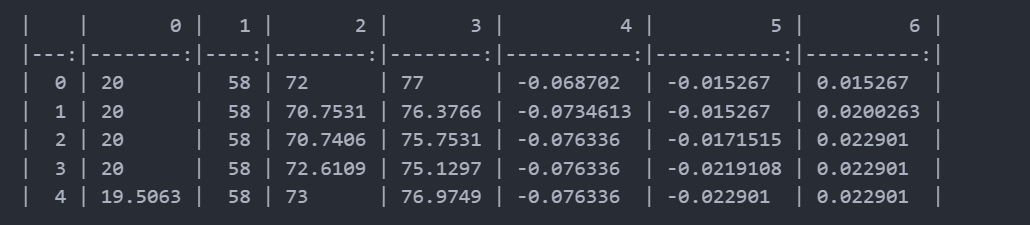
\includegraphics[width=0.8\linewidth]{Images/Improved methods/transfer_learning.png}
        \caption{Dữ liệu sau khi chỉnh sửa}
        \label{fig:interpolation}
    \end{figure}
    \item \textbf{Huấn luyện mô hình:} Mô hình được sử dụng là mô hình cải tiến mà nhóm đã giới thiệu ở trên. Mô hình được huấn luyện trên tập dữ liệu ASL. Weight của mô hình được lưu lại và sử dụng cho việc huấn luyện mô hình trên tập dữ liệu của nhóm.
\end{itemize}